\section{Softwarearchitektur}
\subsection{Komponentenarchitektur}
Die Software ist objektorientiert und modular aufgebaut. Die verschiedenen Teilfunktionen als auch die Harwaretreiber sind in eigene Komponenten eingebettet. Die Komponenten können über eine schmale vordefinierte Schnittstelle angesprochen werden. Im Bild \ref{fig:komponentenmodell} ist das Komponentenmodell abgebildet. 

\begin{figure}[H]
  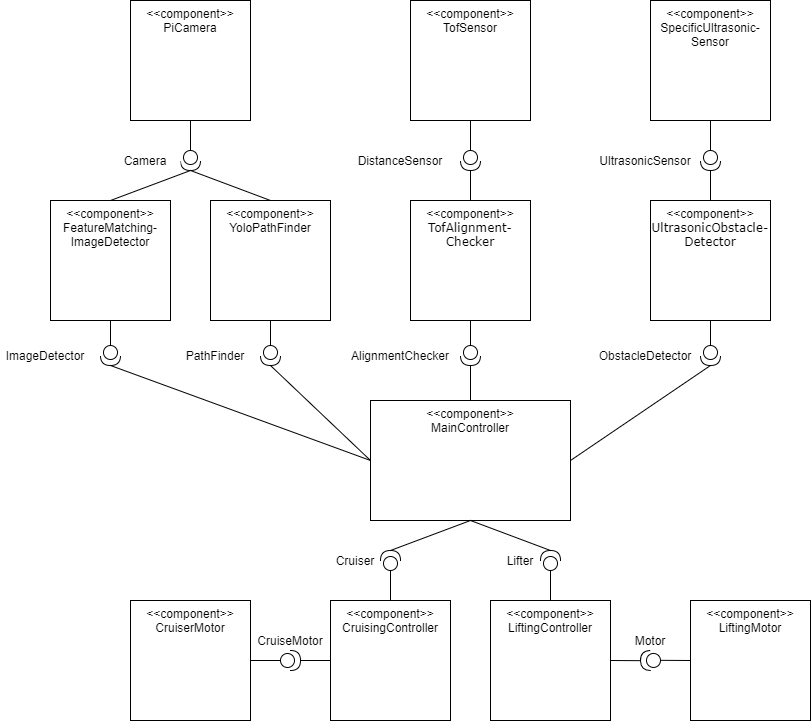
\includegraphics[width=1\textwidth]{img/softwarearchitektur/Softwarearchitektur.png}
  \centering
  \caption{Komponetenmodell}
  \label{fig:komponentenmodell}
\end{figure}

\subsubsection{Main Controller}
Der Main Controller ist der Kern, welche die restlichen Komponenten zielbringend orchestriert. Innerhlab des Main Controllers befindet sich eine Finite State Machine:\\ \texttt{StairClimbingFrog}. Diese ist im Kapitel \ref{sec:fsm} beschrieben. 

In der Abbildung \ref{fig:uml-main} ist zusehen, dass die verschiedenen Zustände und Unterzustände mithilfe von Enumerationen realisiert werden. Dies bring zum einen den Vorteil mit sich, dass man zur Kompilierzeit einen Compileerror erhält, wenn der Zustand nicht existiert. Wären die Zustände mithilfe von Strings realisiert, würde man erst zur Laufzeit erfahren, ob diese Zustände existieren oder nicht. Weiter ist der Workflow dank dem Intellisense, welches durch Enumerationen ermöglicht wird, beschleunigt.

\begin{figure}[H]
  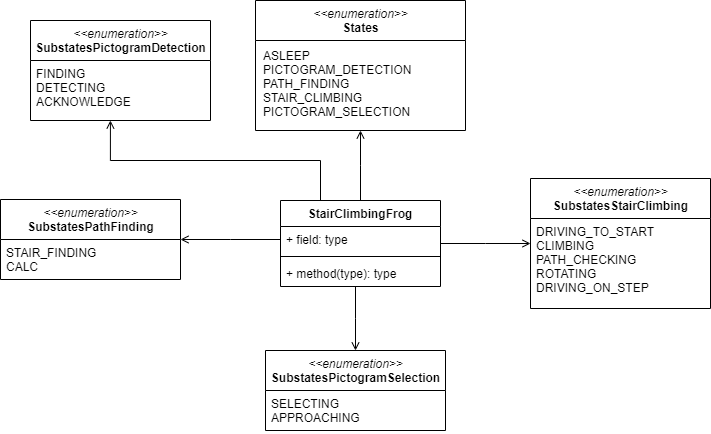
\includegraphics[width=0.95\textwidth]{img/softwarearchitektur/UML-MainController.png}
  \centering
  \caption{UML: MainController}
  \label{fig:uml-main}
\end{figure}


\subsubsection{Lifting Controller}
Der Lifting Controller ist dazu da, den Hauptmotor als auch den Hilfsmotor anzusteuern. Der Hauptmotor steuert die Hubbewegung und mithilfe des Hilfsmotor wird die Stellung der Ausleger bestimmt. 
Das Interface \texttt{LiftingMotor} bestimmt die Methoden welche die Hardwaretreiber-Wrapper: \texttt{MainLiftingMotor} und \texttt{AuxilaryLiftingMotor} implementieren sollen. Der LiftingController implementiert das Interface: \texttt{Lifter}. Über dieses Interface kann der \texttt{LiftingController} von aussen angesprochen werden. Weiter hält er Instanzen der beiden Motoren.

\begin{figure}[H]
  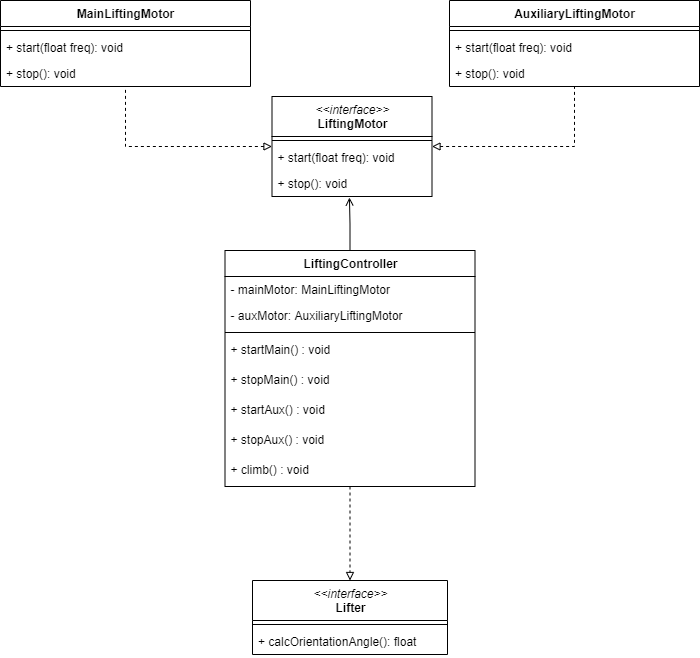
\includegraphics[width=0.95\textwidth]{img/softwarearchitektur/UML-LiftingController.png}
  \centering
  \caption{UML: LiftingController}
  \label{fig:uml-lifting-controller}
\end{figure}


\subsubsection{Cruising Controller}
Die Komponente Cruising Controller ist grundsätzlich gleich aufgebaut wie derLifting Controller. Über das Interface \texttt{CruiseMotor} werden die spezifischen Motorenimplementationen abstrahiert. Der \texttt{CruiseController} hat je eine Instanz vom \texttt{LeftCruiseMotor} und \texttt{RightCruiseMotor}. Über die verschiedenen Methoden welcher durch das \texttt{Cruiser} Interface vorgegeben werden, kann die Fortbewegung des Roboters gesteuert werden.
\begin{figure}[H]
  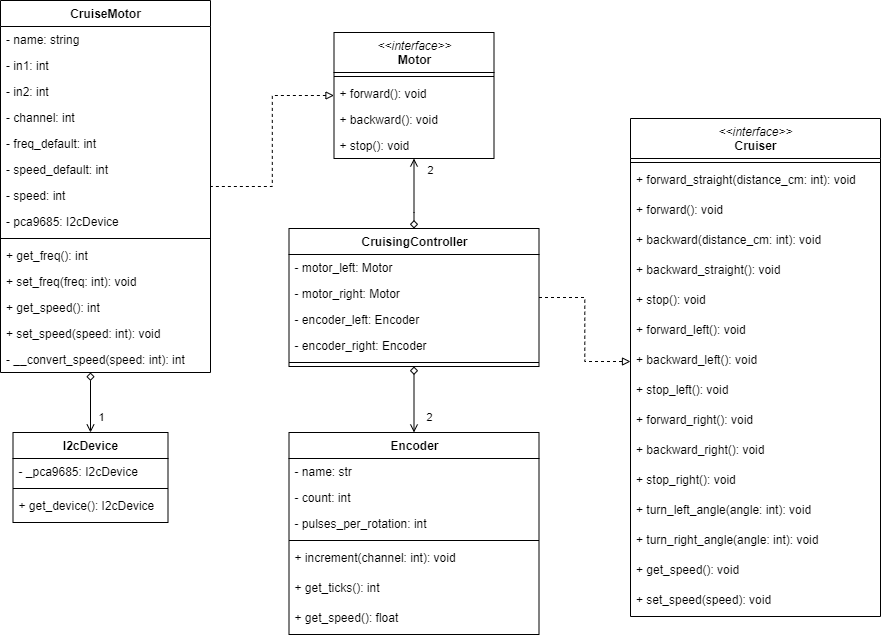
\includegraphics[width=0.95\textwidth]{img/softwarearchitektur/UML-CruisingController.png}
  \centering
  \caption{UML: CruisingController}
  \label{fig:uml-cruising-controller}
\end{figure}

\subsubsection{Tof Alignment Checker}
Dasselbe Spiel beim Tof Alignment Checker. Der \texttt{TofAlignmentChecker} hält die Instanzen der beiden Tof-Treiber-Wrapper \texttt{LeftTofSensor} und \texttt{RightTofSensor} und liefert die Differenz zurück. Mithilfe dieser Differenz kann sich der \texttt{StairClimbingFrog} senkrecht zur Treppe ausrichten.
\begin{figure}[H]
  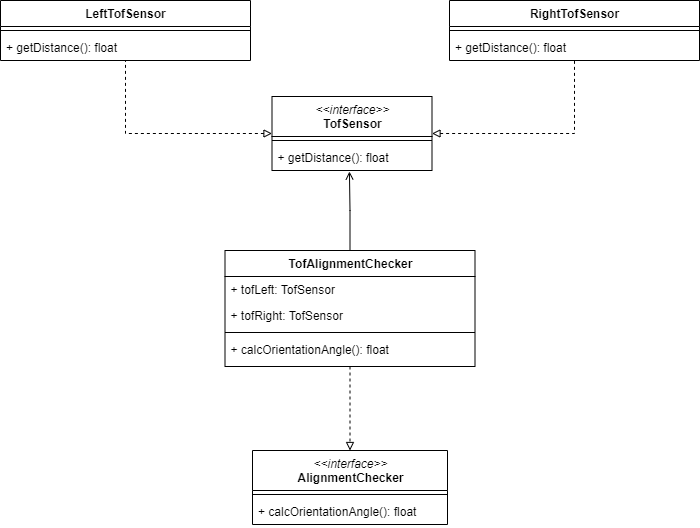
\includegraphics[width=0.95\textwidth]{img/softwarearchitektur/UML-TofAlignmentChecker.png}
  \centering
  \caption{UML: TofAlignmentChecker}
  \label{fig:uml-tof-alignment-checker}
\end{figure}

\subsubsection{Ultrasonic Obstacle Detector}
Wieder ziemlich ähnlich aufgebaut ist der Ultrasonic Obstacle Detector. Über das Interface \texttt{ObstacleDetector} kann der \texttt{UltrasonicObstacleDetector} angesprochen werden. Dieser erkennt mithilfe seiner Instanzen \texttt{FrontUltrasonicSensor} und \texttt{BackUltrasonicSensor} Hindernisse vor und hinter dem Roboter und liefert die Distanz zu diesen zurück.
\begin{figure}[H]
  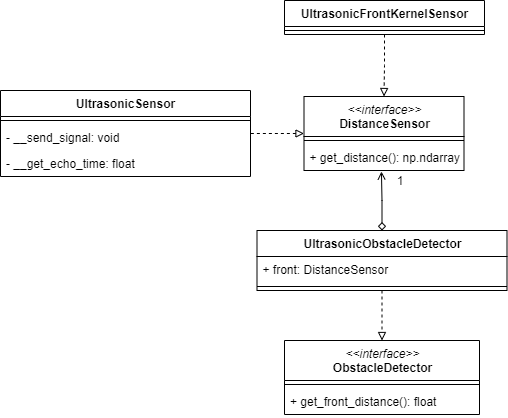
\includegraphics[width=0.95\textwidth]{img/softwarearchitektur/UML-UltrasonicObstacleDetector.png}
  \centering
  \caption{UML: UltrasonicObstacleDetector}
  \label{fig:uml-ultrasonic-obstacle-detector}
\end{figure}

\subsubsection{Feature Matching Image Detector}
\label{sec:architecture-feature-matching}
Die Feature Matchin Image Detector Komponente ist dazu da, das Piktogramm im Startbereich zu finden und zu erkennen. Weiter ist sie dazu da, das richtige Piktogramm im Zielbereich auszuwählen. 
Die Klasse \texttt{Piktogramm} repräsentiert die zu detektierende Piktogramme und deren Keypoints und Deskriptoren (Features). Der \texttt{SiftImageDetector} implementiert über das Interface \texttt{Camera} eine spezifische Kamera Implementation. Für die Bilder, welche mit der Kamera geschossen werden, werden ebenfalls die Features berechnet und mit diesen der Piktogramme abgeglichen. Der Main Controller kann über das \texttt{ImageDetecotr} Interface die entsprechenden Methoden des \texttt{SiftImageDetector} aufrufen.

\begin{figure}[H]
  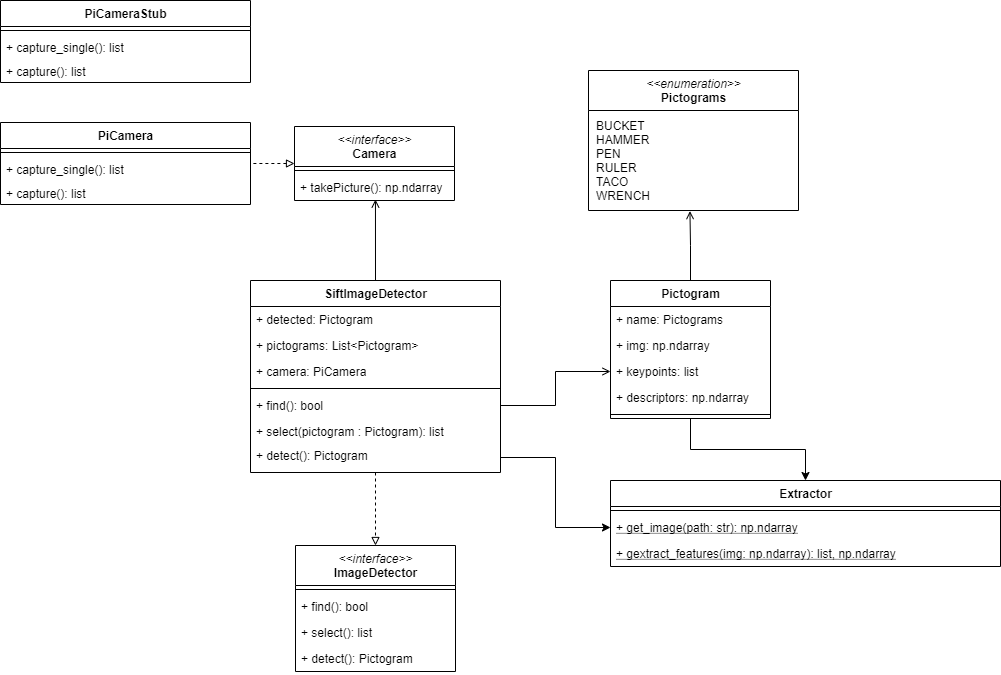
\includegraphics[width=1\textwidth]{img/softwarearchitektur/UML-FeatureMatchingImageDetector.png}
  \centering
  \caption{UML: FeatureMatchingImageDetector}
  \label{fig:uml-feature-matching-image-detector}
\end{figure}

Der \texttt{PiCameraStub} dient lediglich dem Testing. Dem \texttt{SiftImageDetector} kann mittels dependency injection die spezifsiche Kameraimplementation übergeben werden. Die Methoden des Testdoubles liefern vordefinierbare Bilder, welche beim Erzeugen des \texttt{PiCameraStubs} oder danach gesetzt werden können. Im nachfolgenden Codesnippet wird anhand eines Test-Cases die Anwendung des \texttt{PiCameraStubs} veranschaulicht.

\begin{minted}{python}
  class TestSiftImageDetector(unittest.TestCase):
    def test_detect_bucket(self):
        print("\n--- Start test detect bucket ---")
        detectImage = "C:\\git\\hslu-pren\\pren2\\frog\\image_detector\\img\\test\\bucket.jpg"
        selectImage = ""
        stub = PiCameraStub(detectImage, selectImage)
        detector = SiftImageDetector(camera = stub)
        self.assertEqual(detector.detect().name, Pictograms.BUCKET)
    
    ...
 \end{minted}

\subsection{Finite State Machine}
\label{sec:fsm}
Die Main-Komponenten regelt mithilfe einer Finite-State-Machine (FSM) den gessamten Lebenszyklus des Roboters während des Wettbewerbs. In Abbildung \ref{fig:fsm} sind die Hauptzustände modelliert. Innerhalb von jedem Hauptzustand befindet sich eine eigenständige Sub-Statemachine. Die Do-Aktivitäten innerhlab von einem Hauptzusatand werden innerhalb der Unterzustände realisiert. 

\begin{figure}[H]
  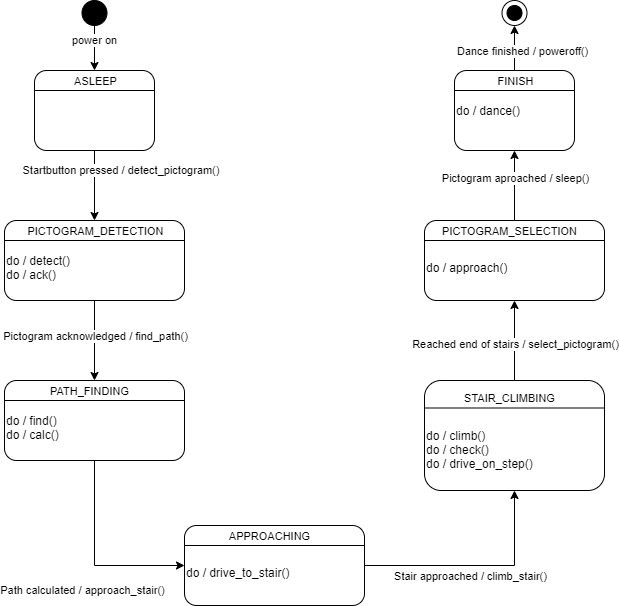
\includegraphics[width=1\textwidth]{img/softwarearchitektur/FSM-FSM.png}
  \centering
  \caption{Finite-State-Machine}
  \label{fig:fsm}
\end{figure}

\begin{figure}[H]
  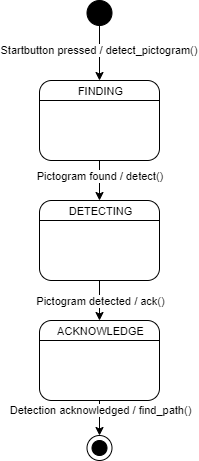
\includegraphics[width=0.40\textwidth]{img/softwarearchitektur/FSM-PICTOGRAM_DETECTION.png}
  \centering
  \caption{FSM: Piktogrammerkennung}
  \label{fig:fsm-pictogrammdetection}
\end{figure}

\begin{figure}[H]
  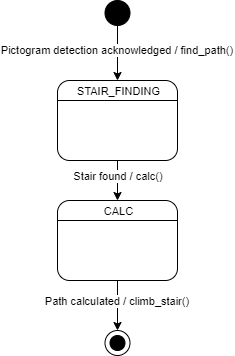
\includegraphics[width=0.40\textwidth]{img/softwarearchitektur/FSM-PATH_FINDING.png}
  \centering
  \caption{FSM: Pfadfindung}
  \label{fig:fsm-pathfinding}
\end{figure}

\begin{figure}[H]
  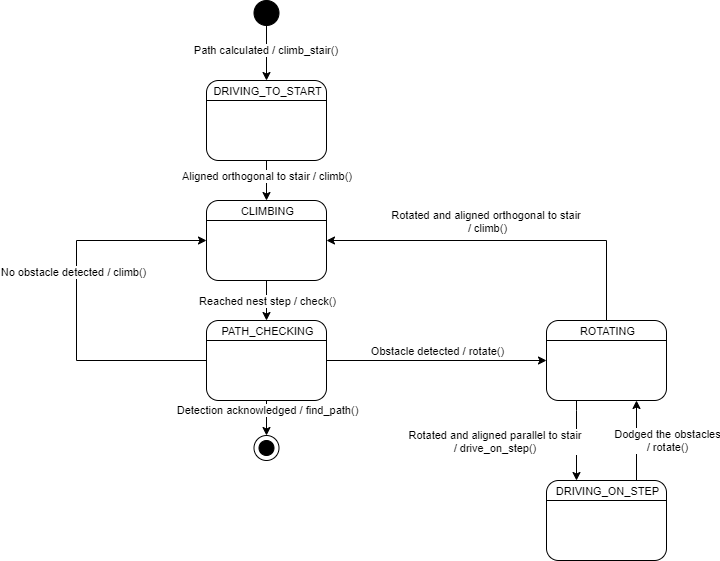
\includegraphics[width=1\textwidth]{img/softwarearchitektur/FSM-STAIR_CLIMBING.png}
  \centering
  \caption{FSM: Treppensteigen}
  \label{fig:fsm-stair-climbing}
\end{figure}

\begin{figure}[H]
  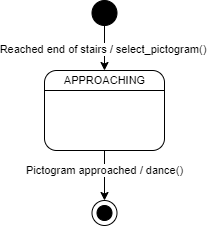
\includegraphics[width=0.40\textwidth]{img/softwarearchitektur/FSM-PICTOGRAM_SELECTION.png}
  \centering
  \caption{FSM: Piktogrammauswahl}
  \label{fig:fsm-pictogram-selection}
\end{figure}













